\chapter{Introduction}
\label{chap:intro}
\textbf{In this section I will explain and summarize what was my internship all about and give a brief outline for the chapters to come.}
\section{Motivation}
	
	As part of my Computer Science Curriculum in the National Engineering School of Tunis, I wanted to complete my internship in a company that is in line with my professional orientation. I did not choose a Telecommunications Company because I wanted to switch to the field of Telecommunications afterwards, but because the mission that was proposed to me was consistent with my professional goals. \\  

	Indeed, my primary mission was to observe the environment and interaction of Tunisie Telecom's employees and their discipline and hard work, I also discovered several new tools and techniques that proved very helpful, I also learned the roles of several devices and also many techniques employed by Tunisie Telecom to guarantee their Networks are top notch, it was a great opportunity for me to actually be in such an environment, which gave me more courage as a student to see myself becoming a Software Engineer. \\
	
	In a second time, I had to design a Web Platform, which is accessible locally. Its role is to enable Tunisie Telecom staff of Creating, Storing, Updating and Deleting different entries of a Fiber Optics stock management program according to their permissions, putting as a priority the simplicity and efficiency of the Web Platform.\\

	Finally,  I'm very satisfied of this internship because it introduced me to a lot of new concepts like HTML, CSS, BootStrap, PHP, MySQL, LAMP stack, Linux and even Git Version Control Systems in a domain that I love. And also allowed me to highlight my skills aquired during my Software Engineering year of studies. \\ 

The place where I did the Internship is shown in Figure~\ref{fig:test1}.
\begin{figure}[ht!]
  \centering
  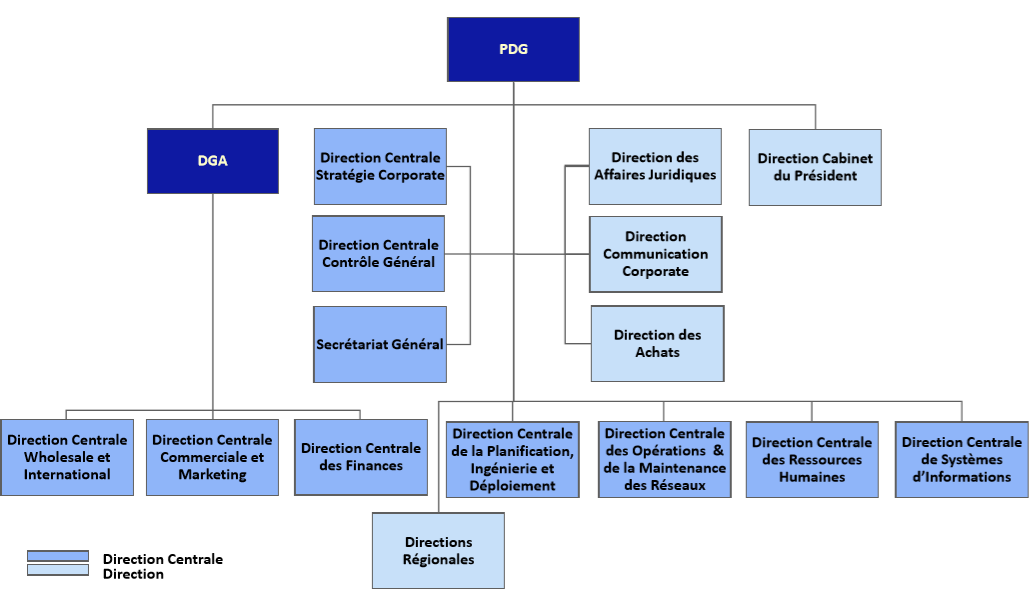
\includegraphics[width=0.6\linewidth]{test_image_goku}
  \caption[Where I Did the Internship]{Tunisie Telecom \index{Goku il-king}}
  \label{fig:test1}
\end{figure}

	This is an Image taken from Google Maps of the Digital Transmission Center (Centre de Transmission Numérique - CTN) of Tunisie Telecom based in Place Pasteur, Belvedere, hereafter noted DTC. Where I did my Internship.
\section{Aims and Objectives - Outline} 
	Besides this Chapter~\autoref{chap:intro} and the Conclusion~\autoref{chap:conc}. There are two main chapters:
	\begin{itemize}
	\item In Chapter~\autoref{chap:org},I will Introduce Tunisie Telecom DTC Belvedere, the company's history and its field of Telecommunications and the things I saw there, as well as the Data Unit (Unité Data) branch, that is responsible for dealing with big companies and clients in which I worked.
	\item In Chapter~\autoref{chap:app}, I will Introduce the Problem that we faced in Tunisie Telecom alongside the Solution I came up with, It's analysis, conception and realisation alongside the tools I learned throughout the way.
	\end{itemize}
